\documentclass[11pt,fleqn]{article}

\textheight=23.3cm
\textwidth=16.5cm
\topmargin=-15mm
\oddsidemargin=0cm

\usepackage{enumerate}
\usepackage{amsmath}
\usepackage{amssymb}
\usepackage{bbm}
\usepackage{ulem}
\usepackage{graphicx}
\usepackage{natbib}
\usepackage{multirow}
\usepackage{xcolor}
\newcommand{\tb}{\hspace*{3mm}}
\bibpunct{(}{)}{;}{a}{,}{,}
\parskip=3mm
\parindent=5mm
\baselineskip=17pt

\usepackage{hyperref}
\hypersetup{
  pdftitle={Acemoglu \& Shimer (2000) - Productivity Gains from Unemployment Insurance},
  pdfauthor={Robert Kirkby},
  colorlinks=true,
  linkcolor=black,
  citecolor=black,
  urlcolor=blue,
  breaklinks=true
}


\begin{document}
\sloppy

%===============================
\newcommand{\rob}[1]{{\noindent\color{blue}\bf #1}}
\newcommand{\robc}[1]{{\noindent\color{blue}\bf R: #1}}
%===============================

\title{Acemoglu \& Shimer (2000) - Productivity Gains from Unemployment Insurance}
\author{Robert Kirkby}
\date{\today}
\maketitle

Brief description of a replication of \cite*{AcemogluShimer2000}, hereafter AS2000. This is not intended as a full description of the model; rather, the goal is to show how the model is expressed in terms of the VFI Toolkit, and to record the choices we had to make where the paper is silent. For a full description see the original paper.

The replication covers the dynamic model: Tables 2--6, Figures 3--6, and the numbers of Section 4.5 (the size of the gains from unemployment insurance, and the bound on the transition costs). Figures 1 and 2 illustrate the static model of Section 2 and are not replicated. Everything is run by \verb|AcemogluShimer2000.m|.

The replication is very close. In Tables 2--5 most entries match the paper's to the reported digit and almost all the rest are within a few units of it, including the tax rate, the fraction of good jobs, unemployment and its duration, all the hours, the consumption drop following job loss, output, leisure and welfare. Table 6 is as close, except the standard deviation of log weekly income, which depends on a handful of workers with near-zero earnings (Section \ref{sec:results}). In two places it is the paper's numbers that seem incorrect: the standard deviation of log annual income, where ours is mostly 0.005--0.010 above the paper's, and the Section 4.5 gains in output and welfare, where ours are about two thirds of the paper's. In both cases our numbers are unchanged when the grid interpolation is refined (Section \ref{sec:results}).


\section{Model description}

Workers are infinitely lived, a period is a week, and there is a single riskless bond with exogenous gross return $R$ and a borrowing constraint $a\geq 0$. Productivity grows at rate $\Gamma$ and everything is normalised by it, so next period's assets are $a' = (R/\Gamma)(a + y - c)$ and the discount factor is $\beta\Gamma^{1-\theta}$. Period utility is
\begin{equation*}
u(c,h) = \frac{(c(\bar{h}-h)^\eta)^{1-\theta}}{1-\theta},
\end{equation*}
($\log c + \eta \log(\bar{h}-h)$ when $\theta=1$), where $h$ is hours spent working or searching.

A worker is in one of four employment states: a good job (wage $w_g$), a bad job (wage $w_b$), unemployed and insured (income $b$), or unemployed and uninsured (no income). Employed workers pay a proportional tax $\tau$ on labour income. An unemployed worker chooses whether to look for a good or a bad job, and finds one with probability $m_g h$ or $m_b h$, where $h$ is search hours. Jobs end with probability $\delta_g$ or $\delta_b$, and the worker becomes insured unemployed. Insured workers who do not find a job lose their eligibility with probability $\phi$. A worker may quit, and is then uninsured. The tax rate $\tau$ balances the government budget, $\tau E[hw] = b \times \text{mass(insured)}$; following AS2000 (fn 12) we take the lowest such $\tau$.

Table 3 sets $\eta=1$ and $\bar{h}=1.7$; Table 4 sets $w_g=1.15$, $m_b=0.15$ and $m_g=0.06$; Table 5 sets $\theta=1$, $w_g=1.15$, $m_b=0.2$ and $m_g=0.04$. In each table the four columns are the benchmark UI policy ($b=0.4$, $\phi=0.04$), High UI ($b=0.44$), Long UI ($\phi=0.036$) and No UI ($b=0$, $\tau=0$). Table 6 adds on-the-job search: bad-job workers choose work hours $h_w$ and search hours $h_s$, and find a good job with probability $m_g h_s$.


\subsection{VFI Toolkit implementation}

The employment state is a semi-exogenous state (\verb|vfoptions.n_semiz=4|), as its transitions depend on the worker's decisions. There is no exogenous shock. There are two decision variables, and both determine the semi-exogenous transitions (\verb|vfoptions.l_dsemiz=2|): search hours $h$, and a binary $s$, which for the unemployed is whether to seek a good job ($s=1$) or a bad one ($s=0$), and for the employed is whether to quit ($s=1$). The transition probabilities are given by \verb|AS2000_SemiExoStateFn.m|.

Employed workers' hours do not affect their transitions, so rather than put work hours on a grid we solve the static first-order condition, eq (6) of AS2000, $\eta c/(\bar{h}-h) = (1-\tau)w$, inside the return function. Substituting the budget constraint gives work hours in closed form given $(a,a')$,
\begin{equation*}
h = \frac{1}{1+\eta}\left(\bar{h} - \eta\frac{a - a'\Gamma/R}{(1-\tau)w}\right),
\end{equation*}
so work hours are exact rather than on a grid. The search hours decision $h$ is then irrelevant for employed workers (a harmless tie). With on-the-job search (Table 6) the $h$ decision is search hours on the job, and work hours solve the same condition with $\bar{h}-h_s$ in place of $\bar{h}$.

Assets are on the paper's grid $\{1.01^n-1\}$ (fn 15), with 396 points up to 49.9, and next period's assets are chosen with the grid interpolation layer (\verb|vfoptions.gridinterplayer=1|, 20 points between grid points), the equivalent of the paper's linear interpolation of the value function. Without it the results are visibly off: near the top of the distribution the weekly saving of a worker in a good job is smaller than the grid spacing, so assets get stuck, and mean assets were 11.6 rather than 16.5. Search hours are on a grid of 101 points on $[0.5,1]$ (on $[0.4,1.4]$ for Table 3, where $\bar{h}=1.7$, and for Table 6 a grid of 151 points that also covers $[0,0.5]$ for search on the job). No column puts mass at the top of the asset grid; the distribution ends at about 35 in the benchmark (the paper reports that no one holds more than 37), and at most at 47.9 (Table 4, No UI).

The tax rate is found by \verb|HeteroAgentStationaryEqm_InfHorz|, starting from the paper's (lowest) tax rate as the initial guess. The statistics come from \verb|EvalFnOnAgentDist_AggVars_InfHorz| on the stationary distribution, except the consumption drop following job loss and the standard deviation of log annual income, which come from a simulated panel (\verb|SimPanelValues_InfHorz|) of 1000 workers for 10,000 weeks, starting from the stationary distribution, pooled over both workers and weeks. Figure 6 is the first worker of that panel. Each table takes 15--25 minutes on one GPU.


\section{Choices where the paper is silent}
\label{sec:choices}

\begin{itemize}
 \item \textbf{Timing.} A quit, and the loss of benefit eligibility, take effect next period, like the other transitions. An insured worker who does not find a job loses eligibility with probability $\phi$, so the probabilities are $m h$, $(1-mh)(1-\phi)$ and $(1-mh)\phi$. With on-the-job search a bad-job worker finds a good job with probability $(1-\delta_b)m_g h_s$, i.e.\ if the bad job does not end first.
 \item \textbf{Quitting good jobs.} We let workers quit good jobs as well as bad ones. No one does.
 \item \textbf{A tiny income for the unemployed.} An uninsured worker with zero assets has no feasible consumption, so their value is $-\infty$. In the paper's continuous-asset model this state is never reached from positive assets, but on a grid it puts a $-\infty$ into the value function, and the expected value next to it can turn into a NaN, which then wrecks the solution (with the grid interpolation layer, every worker chose to consume all their assets). We give the uninsured an income of $10^{-7}$ (and the insured $\max(b,10^{-7})$, so it only matters when $b=0$), which keeps everything finite and, at $10^{-7}$ of a bad-job wage, has no effect on the results. It is not counted as income in any statistic.
 \item \textbf{Leisure} is reported as the mean of $1-h$ rather than $\bar{h}-h$. The two are the same except in Table 3, where $\bar{h}=1.7$, and there only $1-h$ fits the paper's 0.150 (with hours around 0.86). Hours include search hours, so with on-the-job search leisure is $1-h_w-h_s$.
 \item \textbf{Unemployment duration} is the stationary mean completed duration, the unemployment rate divided by the flow into unemployment. This gives the paper's numbers, e.g.\ 2.2 weeks in the No UI column.
 \item \textbf{Std. dev. of log weekly income} is over the employed, of log pre-tax labour income $hw$. It matches Tables 2--5 to the reported digit, except 0.009 against 0.008 in the No UI column of Table 3.
 \item \textbf{Consumption drop following job loss}: over every week in the panel in which an employed worker is laid off (becomes insured unemployed next week; quits are not job loss), the drop is $1-c_{t+1}/c_t$, and we report its mean.
 \item \textbf{Std. dev. of log annual income}: income is after-tax labour income when employed, benefits when insured and zero when uninsured (Section 3 of AS2000), summed over 52-week years, 192 per worker, and the standard deviation is over all worker-years.
 \item \textbf{Welfare} is the consumption $c^*$ that, consumed forever without working (leisure $\bar{h}$), gives the same utility as the average worker in the stationary distribution, $u(c^*,0)/(1-\beta\Gamma^{1-\theta}) = \int V d\mu$.
 \item \textbf{Transition costs} (Section 4.5). Starting from the benchmark stationary distribution, the policy and its tax rate change permanently to those of the High UI (Long UI) column. A worker's problem does not depend on the distribution, so their value function is that of the High UI (Long UI) column, and welfare including the transition is that value function integrated over the benchmark distribution. No transition path needs to be solved.
\end{itemize}


\section{Results}
\label{sec:results}

Each table and figure below shows the paper's original first and ours underneath.

\begin{itemize}
 \item \textbf{Table 2}: most entries match to the reported digit and the rest are close; e.g.\ unemployment is 6.4\%, 6.8\%, 6.6\% and 1.1\% against 6.3\%, 6.7\%, 6.5\% and 1.1\%, and its duration 13.7, 14.5, 14.2 and 2.3 weeks against 13.5, 14.5, 14.0 and 2.2. The largest differences are mean assets in High UI and Long UI (16.5 and 16.8, against 16.8 and 17.0), the fraction of good jobs in High UI (55.2\% against 56.1\%) and with it output (0.935 against 0.938), and search hours of the uninsured in No UI (0.886 against 0.895). The standard deviation of log annual income is 0.175--0.177 against the paper's 0.168--0.171; ours is unchanged when the grid interpolation is refined and comes from a panel of 1000 workers over 10,000 weeks. The thresholds match the paper's (pg 1209--1210): insured workers seek good jobs above assets of 4.1 (paper: about 4), uninsured workers above 9.2 (paper: below 9 they seek bad jobs), and bad-job workers quit above 19.4 (paper: 19). The one qualitative difference is that more generous benefits do not raise mean assets (16.53 in High UI against 16.55 in the benchmark), where the paper has them rise, ``as more workers prepare to undertake the risky search for good jobs'' (pg 1214).
 \item \textbf{Table 3} ($\eta=1$): close throughout, including the sharp fall in the search hours of the insured (0.673, 0.624, 0.664 against 0.672, 0.624, 0.663). Mean assets are up to 0.3 below the paper's, the fraction of good jobs in the benchmark is 51.9\% against 53.0\%, and the consumption drop in the benchmark is 23.4\% against 22.4\%.
 \item \textbf{Table 4} ($w_g=1.15$): close throughout; the fraction of good jobs in the benchmark is 45.8\% against 46.5\%. The standard deviation of log annual income is 0.141--0.144 against the paper's 0.136, and 0.118 against 0.133 with No UI (see the Table 2 bullet).
 \item \textbf{Table 5} ($\theta=1$): close throughout; the fraction of good jobs is 33.8\%, 45.5\% and 37.9\% against 33.8\%, 46.7\% and 38.3\%.
 \item \textbf{Table 6} (on-the-job search): close everywhere except the standard deviation of log weekly income. As the paper describes (pg 1220--1221), most bad-job workers never search, and those whose assets pass a threshold (7.8 in the benchmark) switch from all-work to all-search, with search hours of 0.86; they are about 1\% of the employed, and on average bad-job workers search 0.021 of their time (paper 0.020). Their work hours are tiny but positive, around 0.001, so their log earnings are around $-7$, and these few workers dominate the standard deviation of log weekly income: we get 0.71, against the paper's 0.21. Leaving them out gives 0.128. The paper's number lies between the two, and how it treats these workers is not recoverable; that its own columns vary so much (0.212, 0.208, 0.168, 0.199) is consistent with a statistic driven by a few near-zero earners. (The paper's leisure of 0.862 in the No UI column is presumably a typo.)
 \item \textbf{Section 4.5} (the last table below): UI spending rises by about the paper's amounts, and the transition result replicates: counting the transition, welfare rises only from 0.651 to 0.652 (High UI) and 0.6515 (Long UI), against 0.654 and 0.653 ignoring it. The gains in output and welfare are about two thirds of the paper's (High UI: 0.46\% and 0.40\% against 0.7\% and 0.6\%). These are small differences between columns, and as AS2000 note (pg 1209) the persistence of asset holdings limits the number of significant figures; doubling the points of our grid interpolation layer (10 to 20) did not change ours, so the gap is not numerical error on our side.
 \item \textbf{Figures 3 and 4} replicate the paper's policy functions, including the kink in the consumption of the uninsured at the threshold for seeking good jobs, and the hump in the consumption and the search hours of the insured below assets of 4, where they seek bad jobs. Our search hours are on a grid, so they are step functions.
 \item \textbf{Figure 5}: we show the cumulative distribution as well as the density. The density on a grid is sensitive to numerical error (mass on a single grid point shows up as a spike whose height depends on the grid spacing), whereas the cumulative distribution is not, so the cumulative distribution is the one to compare. About half the mass is below assets of 9, where workers who lose a good job switch to seeking bad jobs, as in the paper, and the distribution ends at about 35 (the paper's ends at about 36). The spike at 9 in the paper's density is a spike in ours too, but ours is taller and narrower, as it sits on a single grid point; the paper's looks to be a histogram with bins of width about one.
 \item \textbf{Figure 6} is very like the paper's: long spells at low assets in bad jobs, with a plateau at about 9, and long climbs to the low 30s in good jobs, followed by rapid falls after a job loss.
\end{itemize}


\section*{Tables}

\begin{table}[h!]
\caption{AS2000 Table 2: results in the benchmark parameterization, and for three alternative UI schemes. Original (top) and replication (bottom). The standard deviation of log annual income differs from the paper's, see Section \ref{sec:results}.}
\label{tab:AS2000_Table2}
\begin{center}
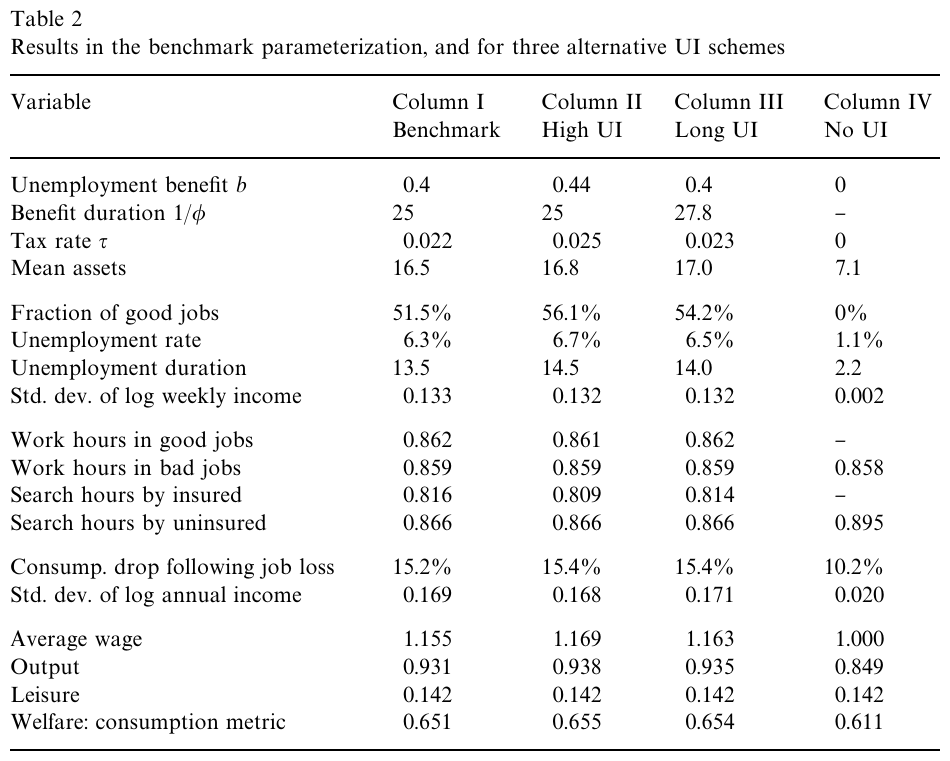
\includegraphics[width=120mm]{./OriginalTablesFigures/AS2000_Table2.png}

\vspace{3mm}
{\small \input{../SavedOutput/LatexInputs/AS2000_Table2.tex}}
\end{center}
\end{table}

\begin{table}[h!]
\caption{AS2000 Table 3: results with a high value of leisure, $\eta=1$. Original (top) and replication (bottom).}
\label{tab:AS2000_Table3}
\begin{center}
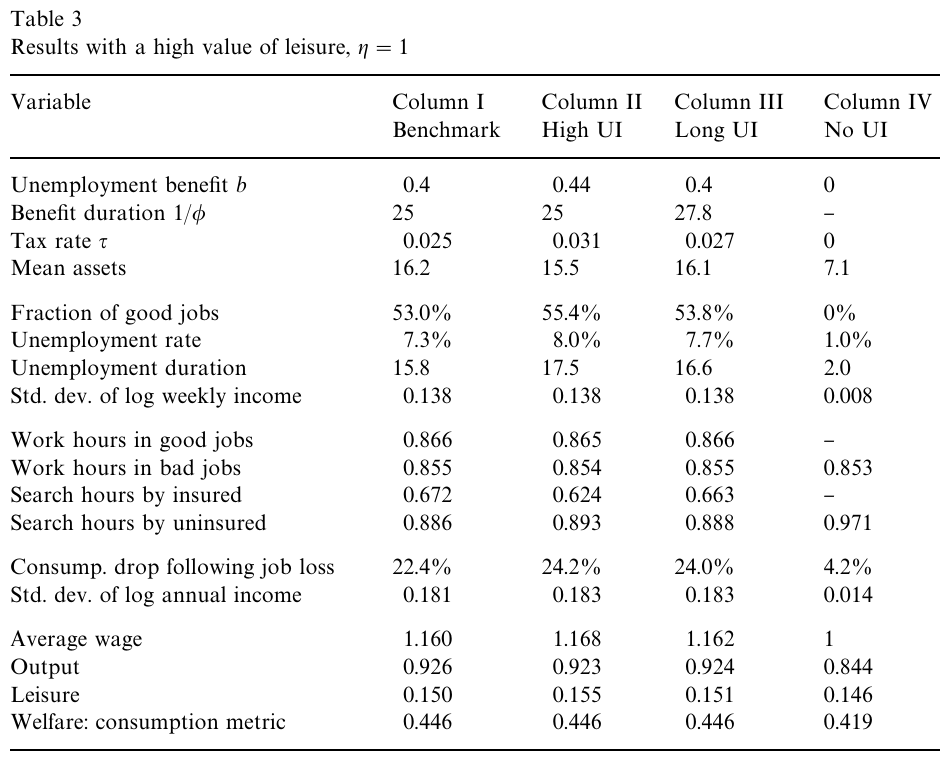
\includegraphics[width=120mm]{./OriginalTablesFigures/AS2000_Table3.png}

\vspace{3mm}
{\small \input{../SavedOutput/LatexInputs/AS2000_Table3.tex}}
\end{center}
\end{table}

\begin{table}[h!]
\caption{AS2000 Table 4: results with low wage dispersion, $w_g=1.15$. Original (top) and replication (bottom). The standard deviation of log annual income differs from the paper's, see Section \ref{sec:results}.}
\label{tab:AS2000_Table4}
\begin{center}
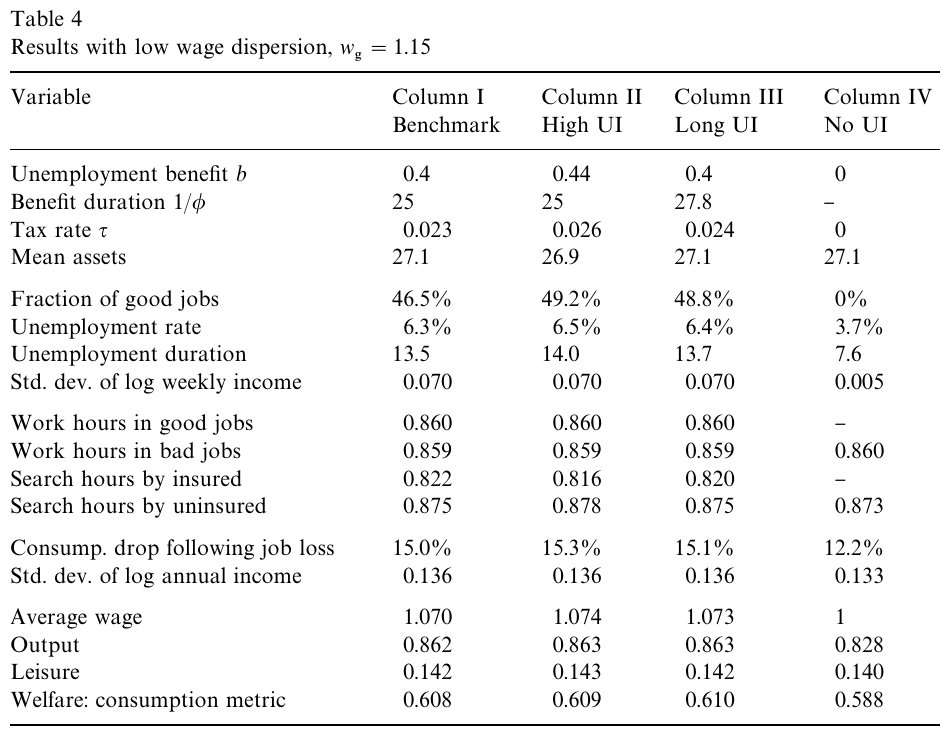
\includegraphics[width=120mm]{./OriginalTablesFigures/AS2000_Table4.png}

\vspace{3mm}
{\small \input{../SavedOutput/LatexInputs/AS2000_Table4.tex}}
\end{center}
\end{table}

\begin{table}[h!]
\caption{AS2000 Table 5: results with low risk aversion, $\theta=1$. Original (top) and replication (bottom).}
\label{tab:AS2000_Table5}
\begin{center}
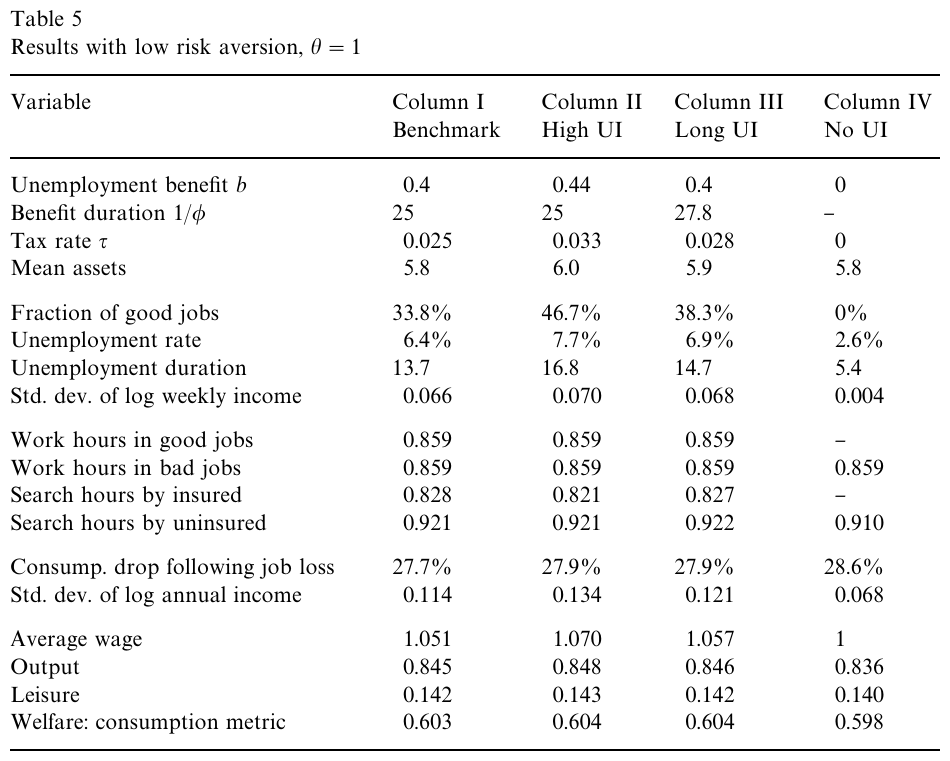
\includegraphics[width=120mm]{./OriginalTablesFigures/AS2000_Table5.png}

\vspace{3mm}
{\small \input{../SavedOutput/LatexInputs/AS2000_Table5.tex}}
\end{center}
\end{table}

\begin{table}[h!]
\caption{AS2000 Table 6: results with on-the-job search. Original (top) and replication (bottom).}
\label{tab:AS2000_Table6}
\begin{center}
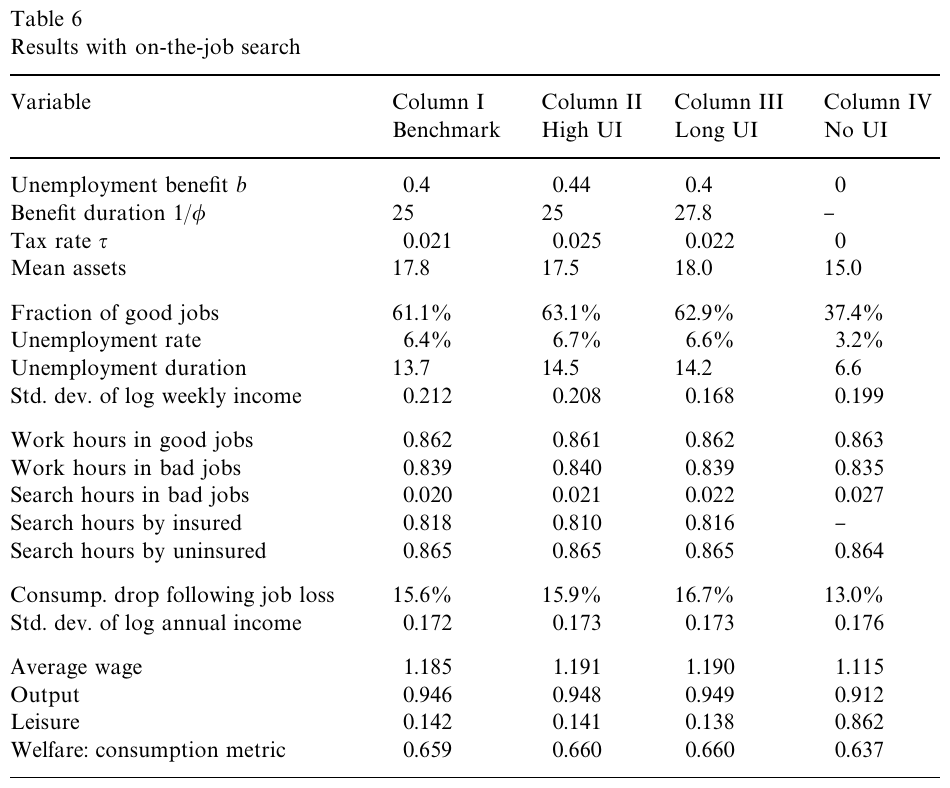
\includegraphics[width=120mm]{./OriginalTablesFigures/AS2000_Table6.png}

\vspace{3mm}
{\small \input{../SavedOutput/LatexInputs/AS2000_Table6.tex}}
\end{center}
\end{table}

\begin{table}[h!]
\caption{AS2000 Section 4.5: the gains from UI relative to the benchmark (Table 2), and welfare including the transition from the benchmark stationary distribution (benchmark welfare \protect\input{../SavedOutput/LatexInputs/AS2000_Section45_benchmarkwelfare.tex}). The paper's numbers, from its text (pg 1215--1216), in brackets; its ratios of the changes in output and UI spending are ``twice'' and ``about four times''.}
\label{tab:Section45}
\begin{center}
{\small \input{../SavedOutput/LatexInputs/AS2000_Section45.tex}}
\end{center}
\end{table}

\clearpage
\section*{Figures}

\begin{figure}[h!]
\caption{AS2000 Figure 3: consumption as a function of normalized assets in the four employment states, benchmark parameterization. Original (top) and replication (bottom). Bad-job consumption is shown only below the assets at which workers quit.}
\label{fig:AS2000_Figure3}
\begin{center}
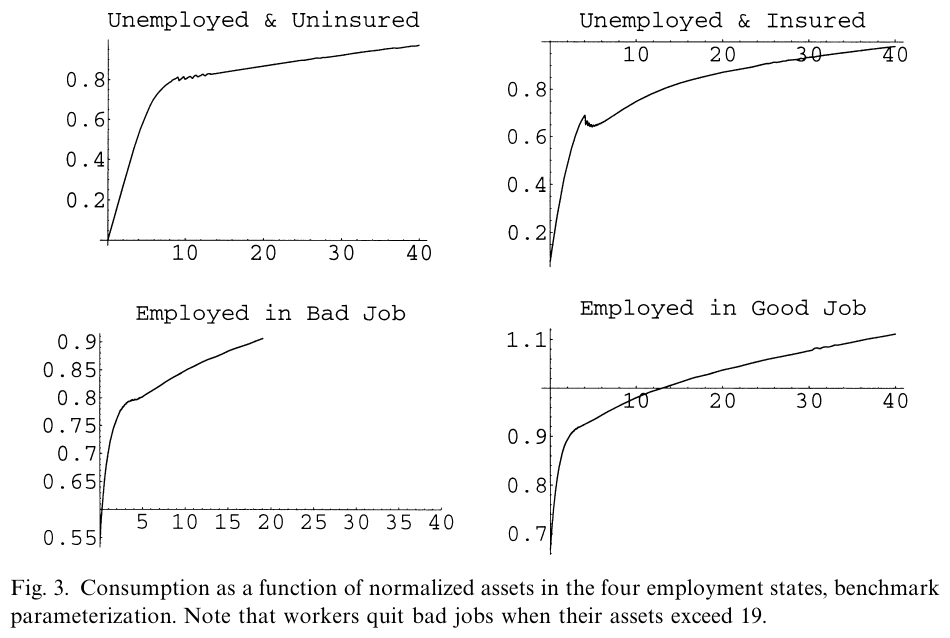
\includegraphics[width=110mm]{./OriginalTablesFigures/AS2000_Figure3.png} \\
\includegraphics[width=140mm]{../SavedOutput/Graphs/AS2000_Fig3.png}
\end{center}
\end{figure}

\begin{figure}[h!]
\caption{AS2000 Figure 4: hours of search or labor supply as a function of normalized assets in the four employment states, benchmark parameterization. Original (top) and replication (bottom).}
\label{fig:AS2000_Figure4}
\begin{center}
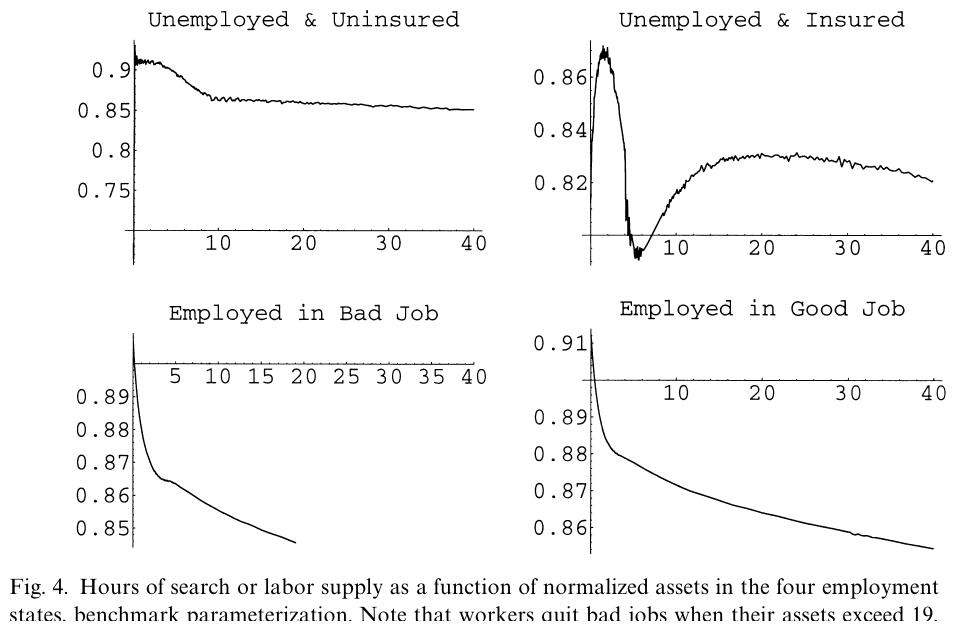
\includegraphics[width=110mm]{./OriginalTablesFigures/AS2000_Figure4.png} \\
\includegraphics[width=140mm]{../SavedOutput/Graphs/AS2000_Fig4.png}
\end{center}
\end{figure}

\begin{figure}[h!]
\caption{AS2000 Figure 5: ergodic distribution of asset holdings, benchmark parameterization. Original (top), and the replication as a cumulative distribution (middle) and as a density (bottom). The density on a grid is sensitive to numerical error, the cumulative distribution is not, so the middle panel is the one to compare.}
\label{fig:AS2000_Figure5}
\begin{center}
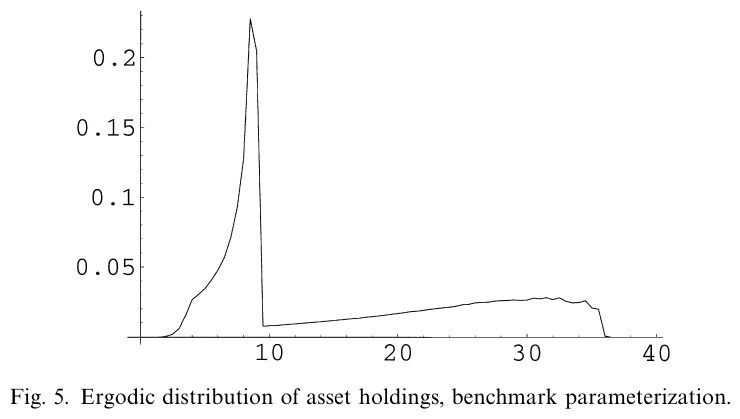
\includegraphics[width=90mm]{./OriginalTablesFigures/AS2000_Figure5.png} \\
\includegraphics[width=120mm]{../SavedOutput/Graphs/AS2000_Fig5cdf.png} \\
\includegraphics[width=80mm]{../SavedOutput/Graphs/AS2000_Fig5.png}
\end{center}
\end{figure}

\begin{figure}[h!]
\caption{AS2000 Figure 6: a typical 10,000 week sample path of asset holdings, benchmark parameterization. Original (top) and replication (bottom, the first worker of the simulated panel).}
\label{fig:AS2000_Figure6}
\begin{center}
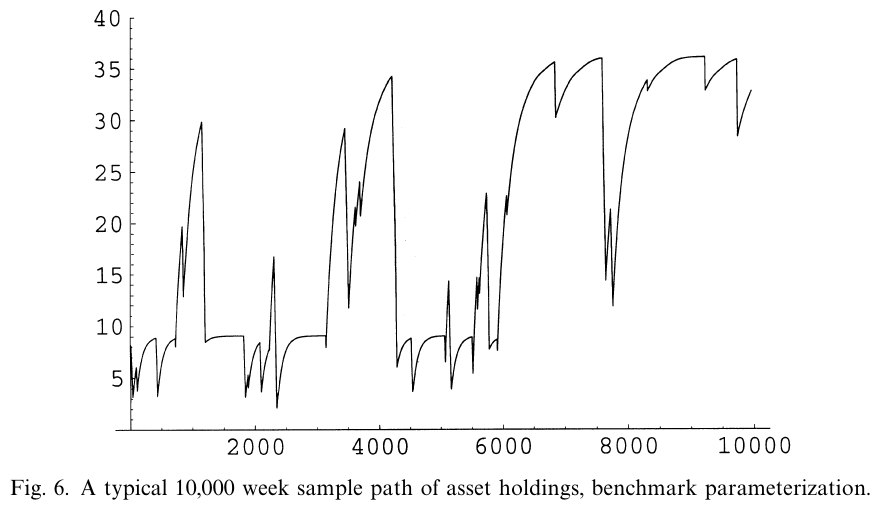
\includegraphics[width=100mm]{./OriginalTablesFigures/AS2000_Figure6.png} \\
\includegraphics[width=130mm]{../SavedOutput/Graphs/AS2000_Fig6.png}
\end{center}
\end{figure}

\clearpage

\bibliographystyle{plainnat}
\bibliography{AS2000refs}

\end{document}
